\documentclass[10pt,a4paper, nocenter]{beamer}
\usetheme{AnnArbor}
\usecolortheme{seahorse}
\usepackage[scaled=0.92]{helvet}
\usepackage[latin1]{inputenc}
\usepackage{blindtext}
\usepackage{amsmath}
\usepackage{appendix}
\usepackage{amsfonts}
\usepackage{amssymb,amsthm}
\usepackage{graphicx}
\usepackage{parskip}
\usepackage{fancyhdr}
\usepackage{lastpage}
\usepackage{enumerate,url}
\usepackage{etoolbox}

\usepackage{caption}
\usepackage{subcaption}

\author[S. Antani]{Sourabh Antani}
\title[Spectral Clustering]{[WORK IN PROGRESS] \\ Research Report - Spectral Clustering}
\date{June 3, 2021}
\institute[SMU - MATH]{Mathematics Department,\\Southern Methodist University}
\begin{document}
	\begin{frame}
		\titlepage
	\end{frame}
    
    \begin{frame}
    \section{Clustering Algorithms}
    \frametitle{Clustering Algorithms}
    Below are some examples of clustering algorithms used in practice, aside from spectral clustering. 
    \begin{itemize}
        \item <1-> Euclidean distance and spatial density based:
	    \begin{itemize}
    	    \item <2-> $k$-means \cite{Macqueen67kmeans} \cite{Lloyd-82-kmeans}
            \item <3-> BIRCH (Balanced Iterative Reducing and Clustering using Hierarchies)\cite{zhang-96-birch}
            \item <4-> Mean-shift \cite{Cheng95meanshift}
            \item <5-> DBSCAN \cite{Ester96adensity-based}
		\end{itemize}
        \item <6-> Linear Algebra based
	    \begin{itemize}
	    	\item <7-> Non-Negative Matrix Factorization \cite{Lawton-1971-nnmf} \cite{Paatero1991-nnmf} \cite{Ding05-nnmf-spectral}
            \item <8-> PCA Based clustering \cite{Zhang-2108-pca}
        \end{itemize}
    \end{itemize}
    \end{frame}

	
	\begin{frame}{Spectral Clustering}
		\framesubtitle{Graph Terminology (1/2)}

		\begin{itemize}
			\item<1-> $\mathbf{G=(V,E)}$ : Undirected graph
			\item<2-> $\mathbf{V=\{v_{1},\dots,v_{n}\}}$: Set of vertices
			\item<3-> $\mathbf{E}$: Set of weighted edges with weight $w_{ij}$ for edge between $v_i$ \& $v_j$. $w_{ij}=0$ iff vertices $v_{i}$ and $v_{j}$ are not connected. $w_{ij}=w_{ji}$. 
			\item<4-> $\mathbf{W=(w_{ij})_{i,j=1,\dots,n}}$ : Weighted \textit{adjacency matrix}
			\item<5-> $\mathbf{d_{i} = \sum_{j=1}^{n}w_{ij}}$: Degree of a vertex $v_i$. 
			\item<6-> $\mathbf{D}$: Degree matrix = $diag(d_{1} ,\dots, d_{n})$. 
			\item<7-> $\mathbf{W(A,B) = \sum_{i\in A, j\in B}w_{ij}}$
		\end{itemize}
	\end{frame}

	\begin{frame}{Spectral Clustering}
		\framesubtitle{Graph Terminology (2/2)}
		
		\begin{itemize}
			\item<1-> $\mathbf{\bar{A}}$: Complement of $A$. 
			\item<2-> $\mathbf{1}_{A}$: Indicator vector = a vector with entries $f_{i} = 1$ if $v_{i} \in A$, $f_{i}=0$ otherwise.
			\item<3-> $\mathbf{\lvert A \rvert}$ : Number of vertices in $A$, one measure of size of $A$
			\item<4-> $\mathbf{vol(A)}$ := $\mathbf{\sum_{i\in A}d_{i}}$: Sum of edge weights, another measure of size of $A$
			\item<5-> $A \subset V$: Connected subset if any two vertices in $A$ can be joined by a path such that all intermediate points also lie in $A$
			\item<6-> Connected Component: $A$ is called \textbf{Connected Component} if it is a connected subset such that $A$ and $\bar{A}$ are disjoint
			\item<7-> \textbf{Partitions} of a graph :Non-empty sets $A_{1},\dots,A_{k}$ form partition of graph if $A_{i} \cap A_{j} = \emptyset$ and $A_{1}\cup \dots \cup A_{k} = V$
			
		\end{itemize}
	\end{frame}


	\begin{frame}{Spectral Clustering}
		\framesubtitle{Graph Laplacians}
		\begin{center}

			\begin{tabular}{|c|c|c|}
				\hline
				Unnormalized & Normalized (Symmetric) & Normalized (Random Walk)\\
				\hline
				$L = D-W$ & $L_{sym} = D^{-1/2}LD^{-1/2} $ & $L_{rw} = D^{-1}L$ \\
				 & =$ I - D^{-1/2}WD^{-1/2}$ & = $I - D^{-1}W$\\
				\hline
				Symmetric & Symmetric & Not-Symmetric \\
				\hline
				$u$ - eigenvector & $D^{1/2}u$ - eigenvector &  $u$ - eigenvector\\
				\hline
				\multicolumn{3}{|c|}{Positive-semidefinte, Non-Negative Real-Valued Eigenvalues}\\
				\hline
				\multicolumn{3}{|c|}{0 is an eigenvalue with multiplicity equal to no. of connected components}\\
				\hline
			\end{tabular}
		\end{center}
	\end{frame}


	\begin{frame}{Spectral Clustering}
		\framesubtitle{Graph Cuts}
		\begin{itemize}
			\item<1-> The goal of clustering is to maximize the similarity within cluster and minimize the similarity between clusters.
			\item<2-> Minimizing the between cluster similarity equals to minimizing the objective function $$  \text{cut}(A_{1}, \dots, A_{k}) := \frac{1}{2}\sum_{i-1}^{k}W(A_i,\bar{A}_{i}) $$
			\item<3-> To maximize the within-cluster similarity, we define two objective functions \begin{align} RatioCut(A_{1},\dots,A_{k}) &= \frac{1}{2} \sum_{i=1}^{k}\frac{W(A_{i},\bar{A}_{i})}{\lvert A_{i} \rvert}
			= \sum_{i=1}^{k}\frac{cut(A_{i},\bar{A}_{i})}{\lvert A_{i} \rvert} \\
			Ncut(A_{1},\dots,A_{k}) &= \frac{1}{2}\sum_{i=1}^{k}\frac{W(A_{i},\bar{A}_{i})}{vol(A_{i})} = 
			\sum_{i=1}^{k}\frac{cut(A_{i},\bar{A}_{i})}{vol(A_{i})} \end{align}
			
		\end{itemize}
	\end{frame}

	\begin{frame}{Spectral Clustering}
		\framesubtitle{Algorithms - Unnormalized Spectral Clustering}
    \begin{algorithm}[H]
		\DontPrintSemicolon
		\KwIn{Similarity matrix $S \in \mathbb{R}^{n\times n}$, number $k$ of clusters to construct.}
		\Begin{
			Construct a similarity graph and its weighted adjacency matrix $W$\;
			Compute the unnormalized Laplacian $L$\;
			Compute the first $k$ eigenvectors $u_{1},\dots, u_{k} $ of $L$\;
			Let $U \in \mathbb{R}^{n\times k}$ be the matrix containing the vectors $u_{1},\dots, u_{k}$ as columns\;
			For $i = 1,\dots, n$, let $y_{i} \in \mathbb{R}^k$ be the vector corresponding to the $i^{th}$ row of $U$\;
			Cluster the points $(y_{i}), i=1,\dots,n$ in $\mathbb{R}^k$ with the k-means algorithm into clusters
			$C_{1},\dots, C_{k}$\;}
		\KwOut{Clusters $A_{1},\dots, A_{k}$ with $A_{i} = \{x_{j}| y_{j} \in C_{i}\}$}

	\end{algorithm}


	\end{frame}

	\begin{frame}{Spectral Clustering}
	\framesubtitle{Algorithms - Normalized Spectral Clustering - Shi \& Malik (2000) \cite{Shi-Malik-maxcut-00}}
	\textit{This algorithm uses generalized eigenvectors of L, which are the eigenvectors of normalized random-walk Laplacian $L_{rw}$}
	\begin{algorithm}[H]
		\DontPrintSemicolon
		\KwIn{Similarity matrix $S \in \mathbb{R}^{n\times n}$, number $k$ of clusters to construct}
		\Begin{
			Construct a similarity graph and its weighted adjacency matrix $W$\;
			Compute the unnormalized Laplacian $L$.\;
			Compute the first $k$ generalized eigenvectors $u_{1},\dots, u_{k} $ of generalized eigenproblem $Lu = \lambda Du$.\;
			Let $U \in \mathbb{R}^{n\times k}$ be the matrix containing the vectors $u_{1},\dots, u_{k}$ as columns.\;
			For $i = 1,\dots, n$, let $y_{i} \in \mathbb{R}^k$ be the vector corresponding to the $i^{th}$ row of $U$.\;
			Cluster the points $(y_{i}), i=1,\dots,n$ in $\mathbb{R}^k$ with the k-means algorithm into clusters $C_{1},\dots, C_{k}$.\;
		}
		\KwOut{Clusters $A_{1},\dots, A_{k}$ with $A_{i} = \{x_{j}| y_{j} \in C_{i}\}$}
	\end{algorithm}

	\end{frame}

	\begin{frame}{Spectral Clustering}
	\framesubtitle{Algorithms - Normalized Spectral Clustering - Ng, Jordan \& Weiss (2002) \cite{ng-jordan-01}}
		\textit{This algorithm uses the eigenvectors of normalized symmetric Laplacian $L_{sym}$. Note that if $D^{1/2}u$ is an eigenvector of $L_{sym}$ if $u$ is an eigenvector of $L$ hence an additional normalization step is needed.}
	
	\begin{algorithm}[H]
		\DontPrintSemicolon
		\KwIn{Similarity matrix $S \in \mathbb{R}^{n\times n}$, number $k$ of clusters to construct.}
		\Begin{
			Construct a similarity graph and its weighted adjacency matrix $W$\;
			Compute the normalized Laplacian $L_{sym}$\;
			Compute the first $k$ eigenvectors $u_{1},\dots, u_{k} $ of $L_{sym}$\;
			Let $U \in \mathbb{R}^{n\times k}$ be the matrix containing the vectors $u_{1},\dots, u_{k}$ as columns\;
			Form the matrix $T \in \mathbb{R}^{n\times k}$ from $U$ by normalizing the norm to 1, $t_{ij} = u_{ij}/(\sum_{k}u_{ik}^2)^{1/2}$\;
			For $i = 1,\dots, n$, let $y_{i} \in \mathbb{R}^k$ be the vector corresponding to the $i^{th}$ row of $U$\;
			Cluster the points $(y_{i}), i=1,\dots,n$ in $\mathbb{R}^k$ with the k-means algorithm into clusters $C_{1},\dots, C_{k}$\;
		} 
		\KwOut{Clusters $A_{1},\dots, A_{k}$ with $A_{i} = \{x_{j}| y_{j} \in C_{i}\}$}
	\end{algorithm}
	\end{frame}

	\begin{frame}{Spectral Clustering}
		\framesubtitle{Numerical Experiments}
		Mixture of 4 Gaussians in $\mathbb{R}^1$ with a Gaussian kernel $e^{-\lvert x_i - x_j \rvert^2/(2\sigma^2)}$ with $\sigma = 1$ as similarity function.
		\begin{figure}[h]
			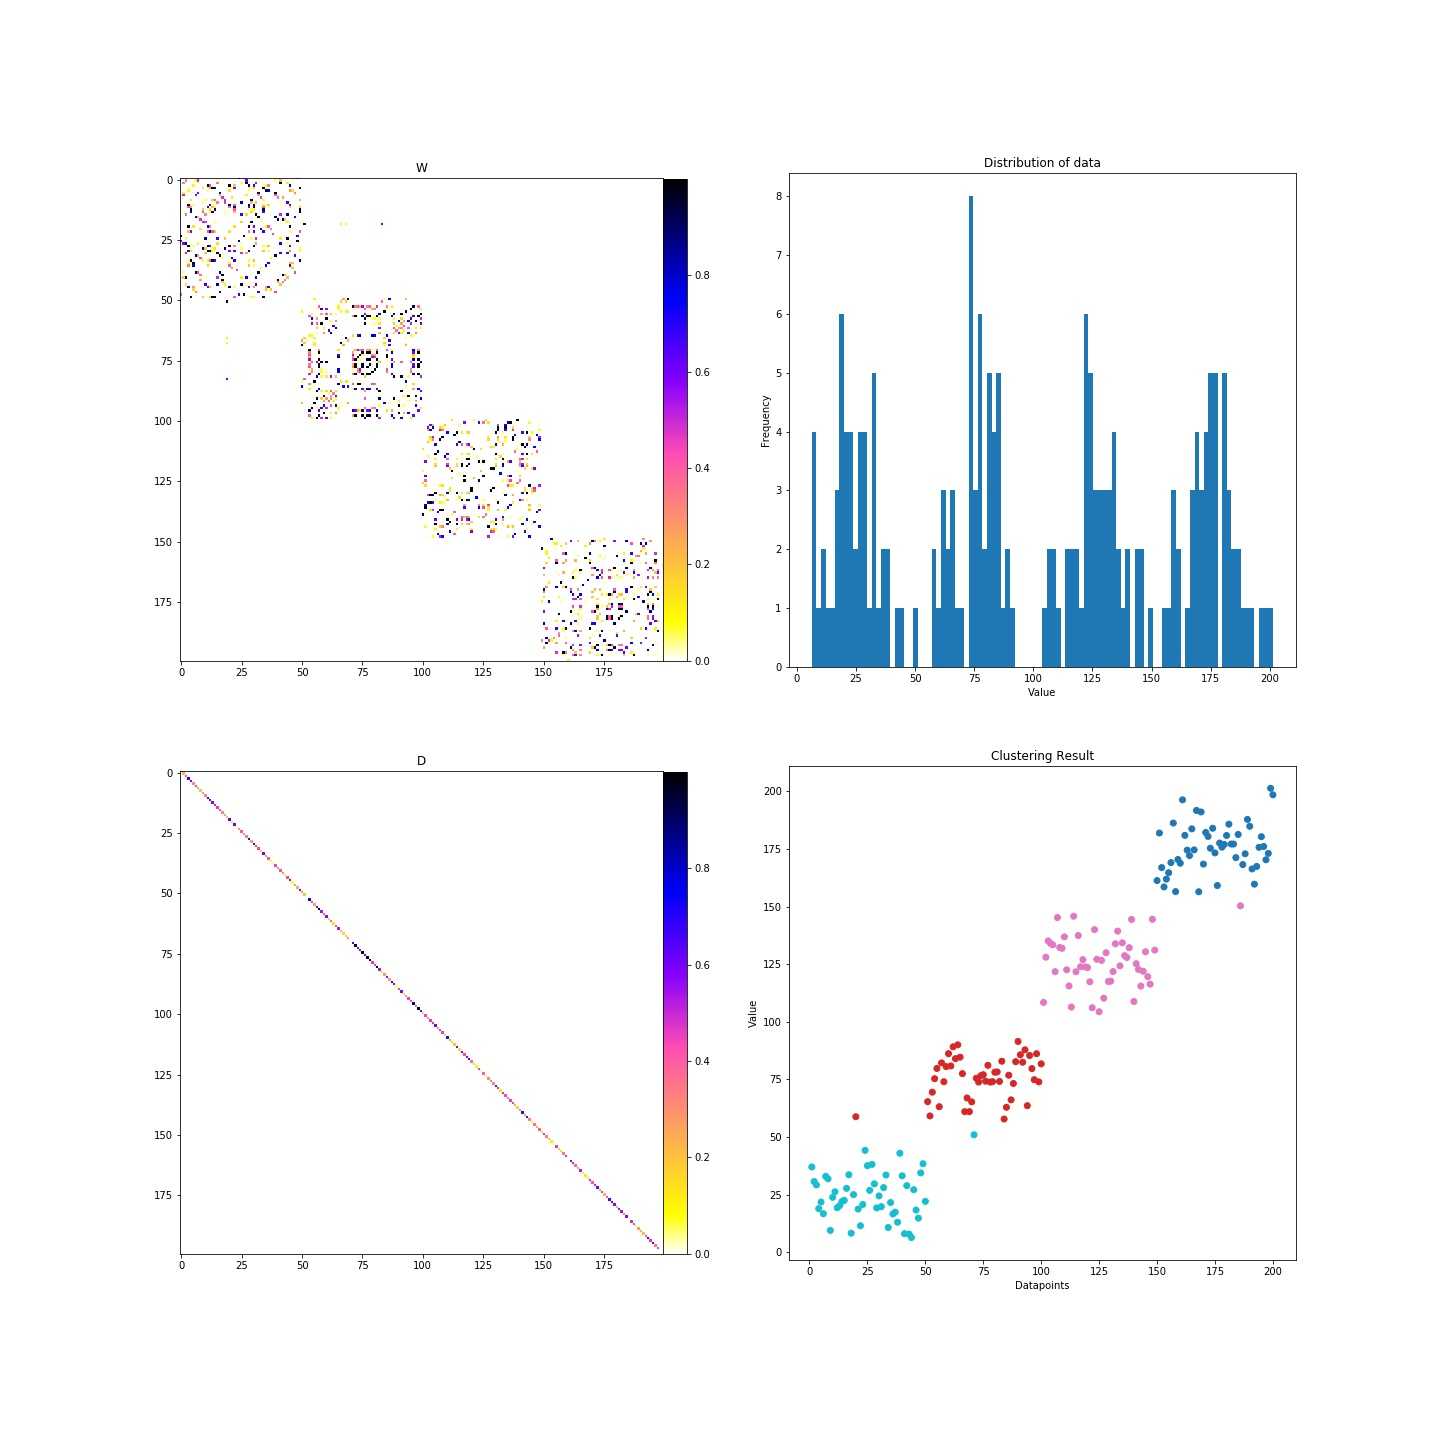
\includegraphics[height=0.6\textheight]{../../images/1DCluster.jpg}
			\caption{Clustering results for 200 points in $\mathbb{R}^1$}
			\label{fig:1dresults}
		\end{figure}
	\end{frame}

	\begin{frame}{Spectral Clustering}
		\framesubtitle{Numerical Experiments}
		Points in $\mathbb{R}^2$ with $\lvert\lvert x-y \rvert\rvert_2$ as similarity function
		\begin{figure}[h]
        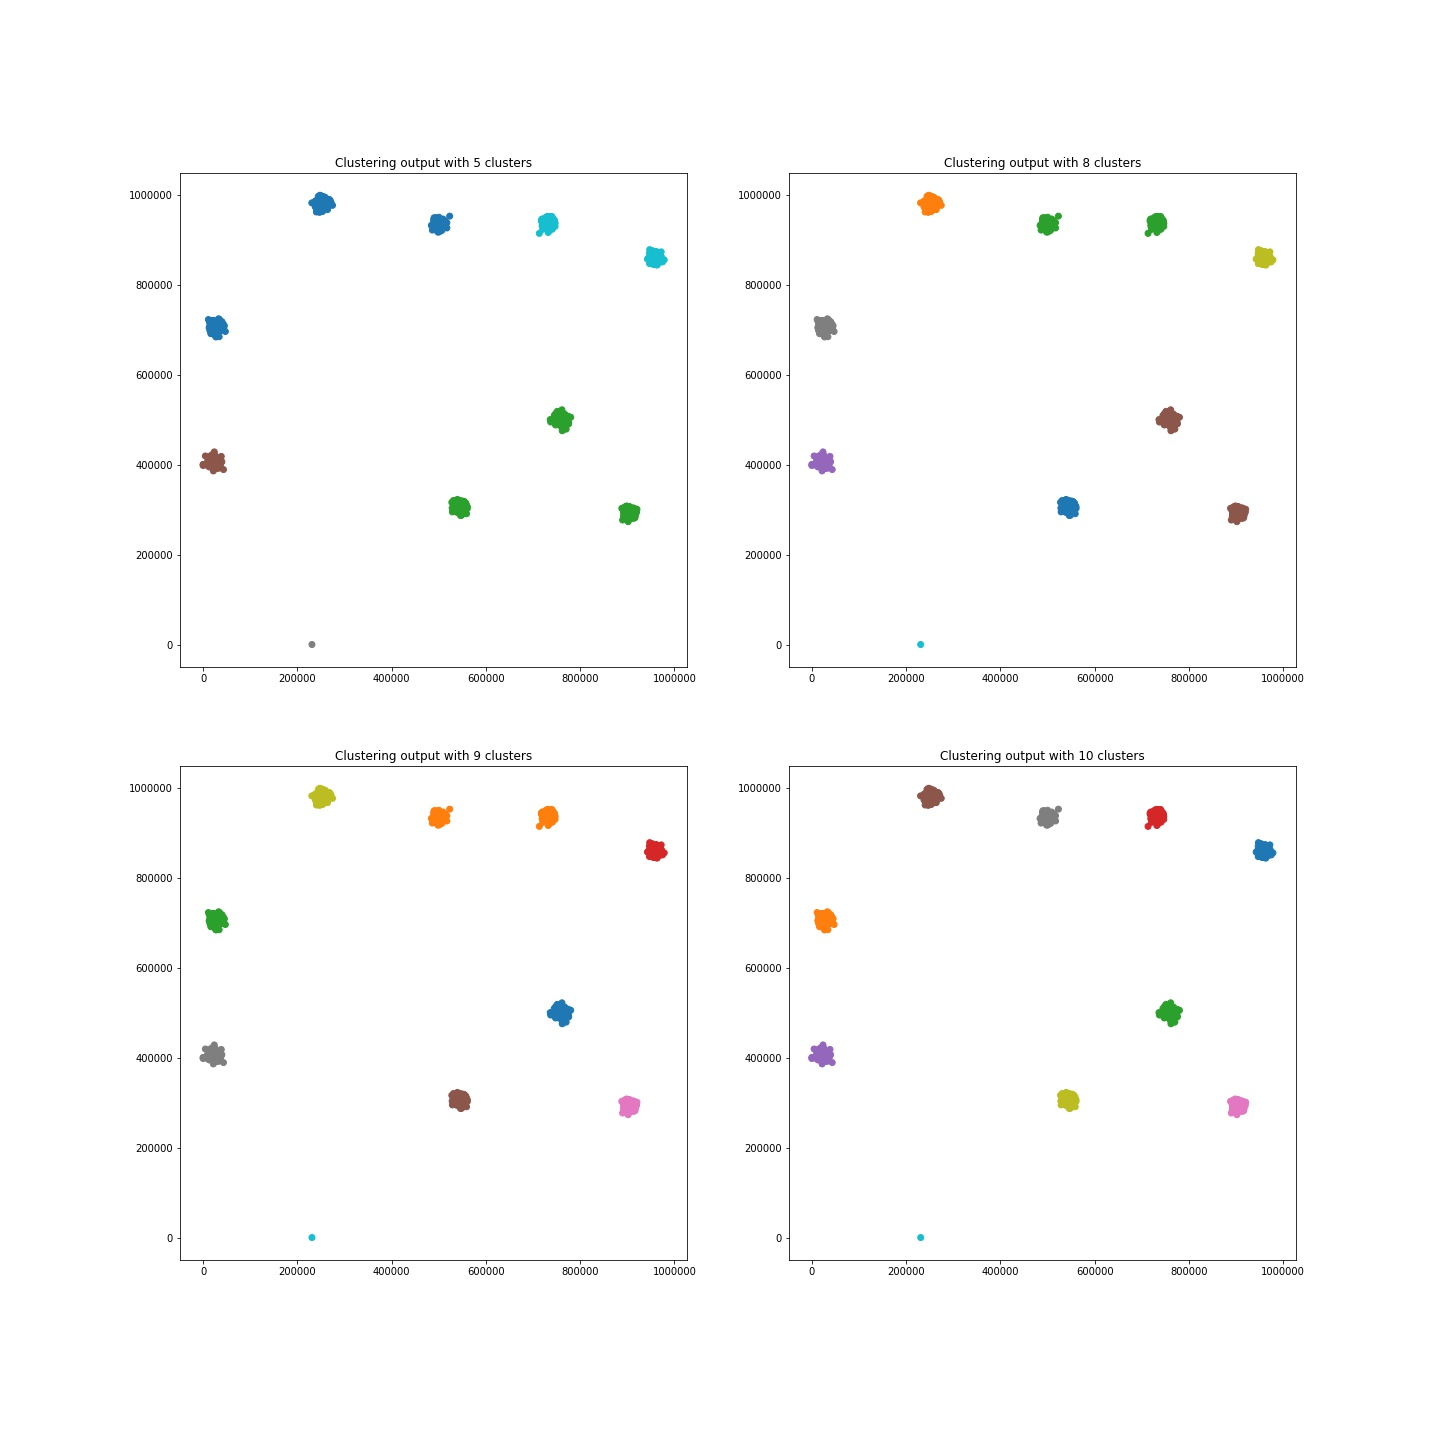
\includegraphics[height=0.65\textheight]{../../images/2DCluster.jpg}
		\caption{Clustering results for 1351 points in $\mathbb{R}^2$}
		\label{fig:2dresults}
		\end{figure}
	\end{frame}
	
	\begin{frame}{Spectral Clustering}
		\framesubtitle{Numerical Experiments}
		Unsupervised Image Classification
        \begin{figure}[h]
			\begin{center}
				\begin{subfigure}[b]{0.3\textwidth}
					\centering
					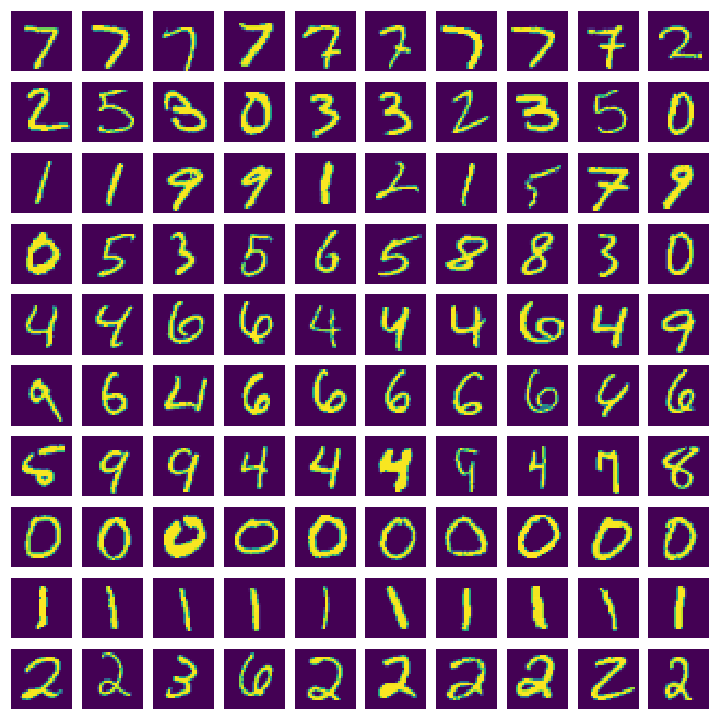
\includegraphics[width=\textwidth]{../../images/number_clustering_10_0norm.png}
					\caption{Count of pixels that are non-zero in both images as similarity measure}
					\label{fig:clustering_10_0norm}
				\end{subfigure}           
				\begin{subfigure}[b]{0.3\textwidth}
					\centering
					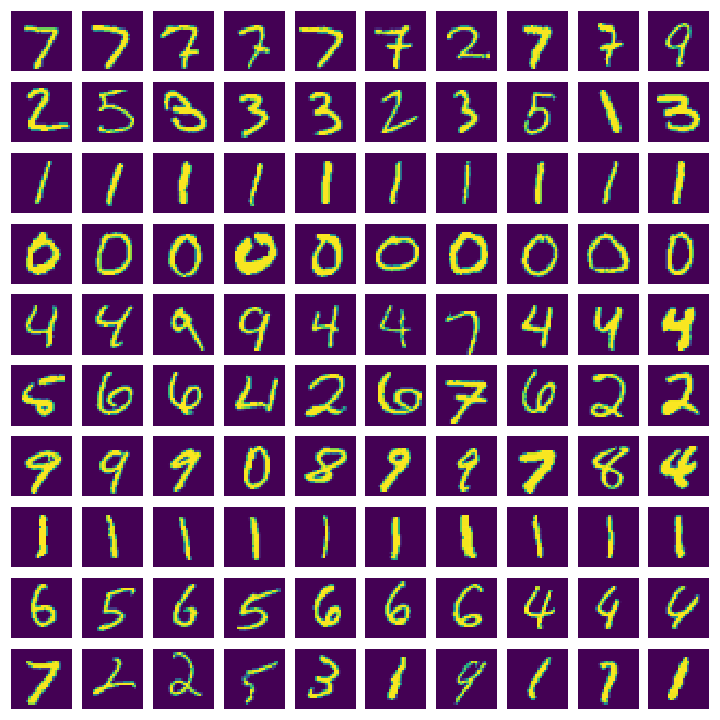
\includegraphics[width=\textwidth]{../../images/number_clustering_10_2norm.png}
					\caption{Inverse of 2-norm of the difference vector between two images as similarity measure}
					\label{fig:clustering_10_2norm}
				\end{subfigure}           
				\begin{subfigure}[b]{0.3\textwidth}
					\centering
					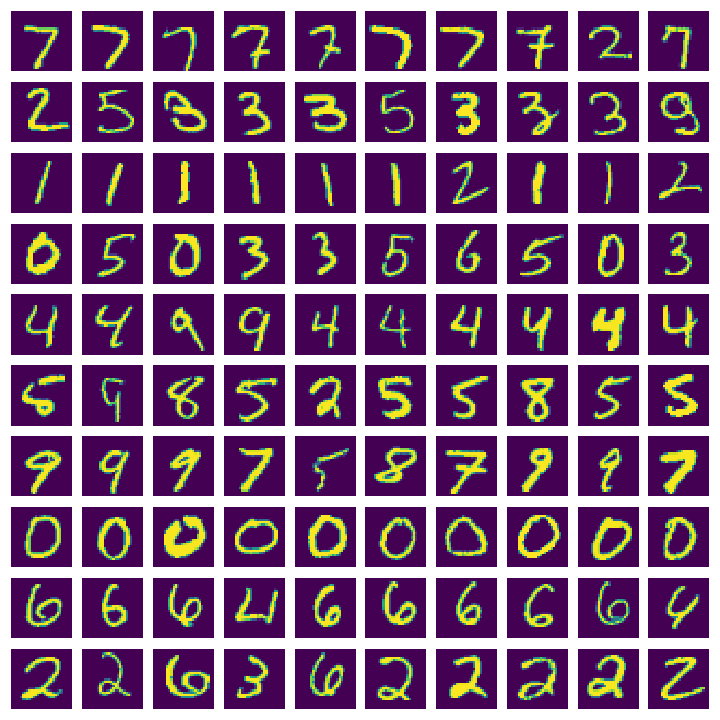
\includegraphics[width=\textwidth]{../../images/number_clustering_10_hamming.png}
					\caption{Count of pixels that are zero or non-zero in both images as similarity measure}
					\label{fig:clustering_10_hamming}
				\end{subfigure}           
			\end{center}
			\caption{2000 images from MNIST data-set were clustered into 10 clusters. In the above figure, each row of images represent a cluster and show the first 10 images in that cluster}
			\label{fig:mnist10ClusterImages}
		\end{figure}

	\end{frame}

	\begin{frame}{Spectral Clustering}
	\framesubtitle{Numerical Experiments}
	Unsupervised Image Classification
        \begin{figure}[h]
		\begin{center}
			\begin{subfigure}[b]{0.3\textwidth}
				\centering
				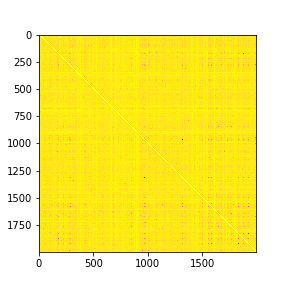
\includegraphics[width=\textwidth]{../../images/w_0norm.png}
				\caption{Count of pixels that are non-zero in both images as similarity measure}
				\label{fig:w_0norm}
			\end{subfigure}           
			\begin{subfigure}[b]{0.3\textwidth}
				\centering
				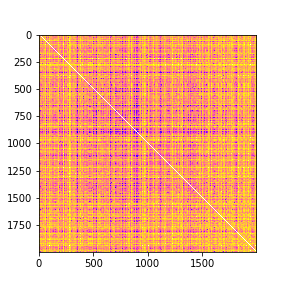
\includegraphics[width=\textwidth]{../../images/w_2norm.png}
				\caption{Inverse of 2-norm of the difference vector between two images as similarity measure}
				\label{fig:w_2norm}
			\end{subfigure}           
			\begin{subfigure}[b]{0.3\textwidth}
				\centering
				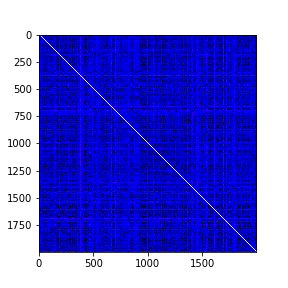
\includegraphics[width=\textwidth]{../../images/w_hamming.png}
				\caption{Count of pixels that are zero or non-zero in both images as similarity measure}
				\label{fig:w_hamming}
			\end{subfigure}           
		\end{center}
		\caption{Weighted adjecency matrix for 2000 images from MNIST data-set with similarity functions described under the images}
		\label{fig:mnistWImages}
	\end{figure}
	
	\end{frame}
	
	
	\begin{frame}{Spectral Clustering}
	\framesubtitle{Numerical Experiments}
	Unsupervised Image Classification
	\begin{figure}[h]
		\begin{center}
			\begin{subfigure}[b]{0.4\textwidth}
				\centering
				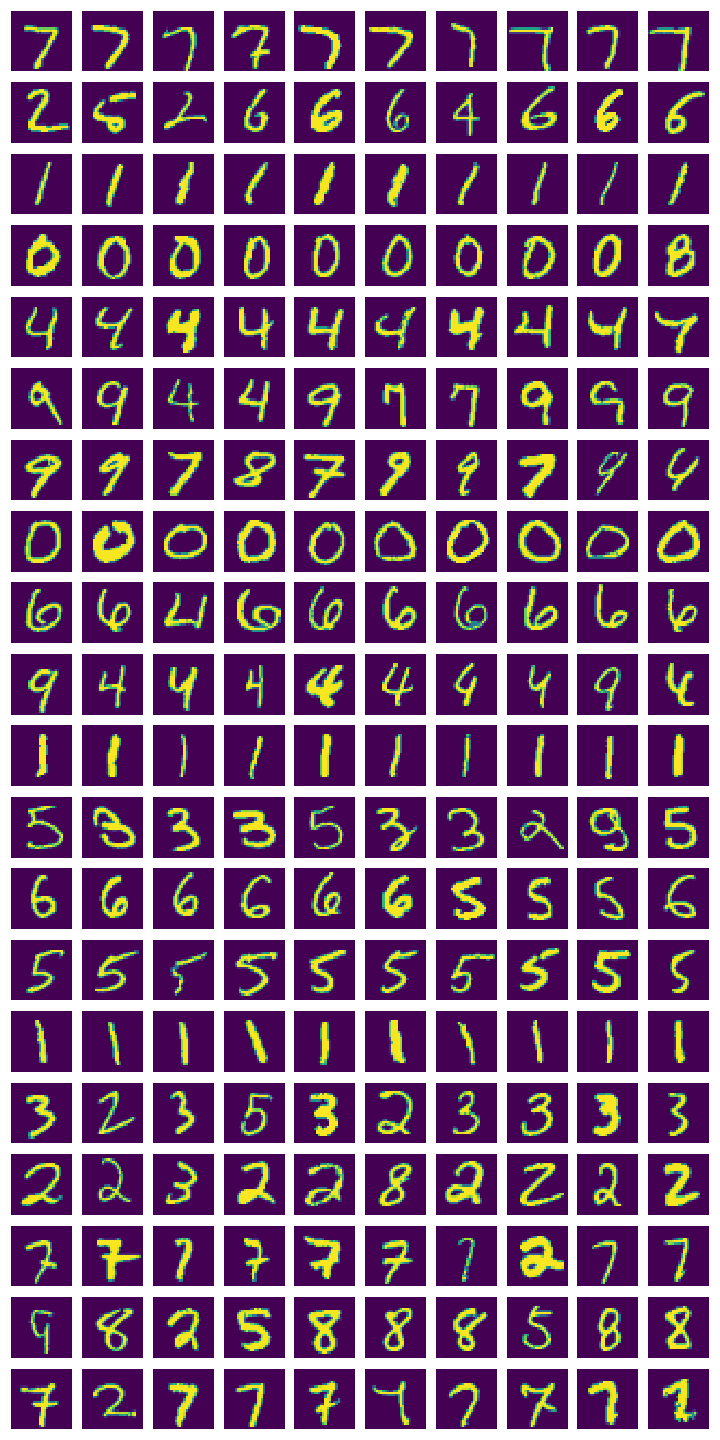
\includegraphics[height={0.6\textheight}]{../../images/number_clustering.png}
				\caption{Count of pixels that are non-zero in both images as similarity measure}
				\label{fig:clustering_20_0norm}
			\end{subfigure}
			\begin{subfigure}[b]{0.4\textwidth}
				\centering
				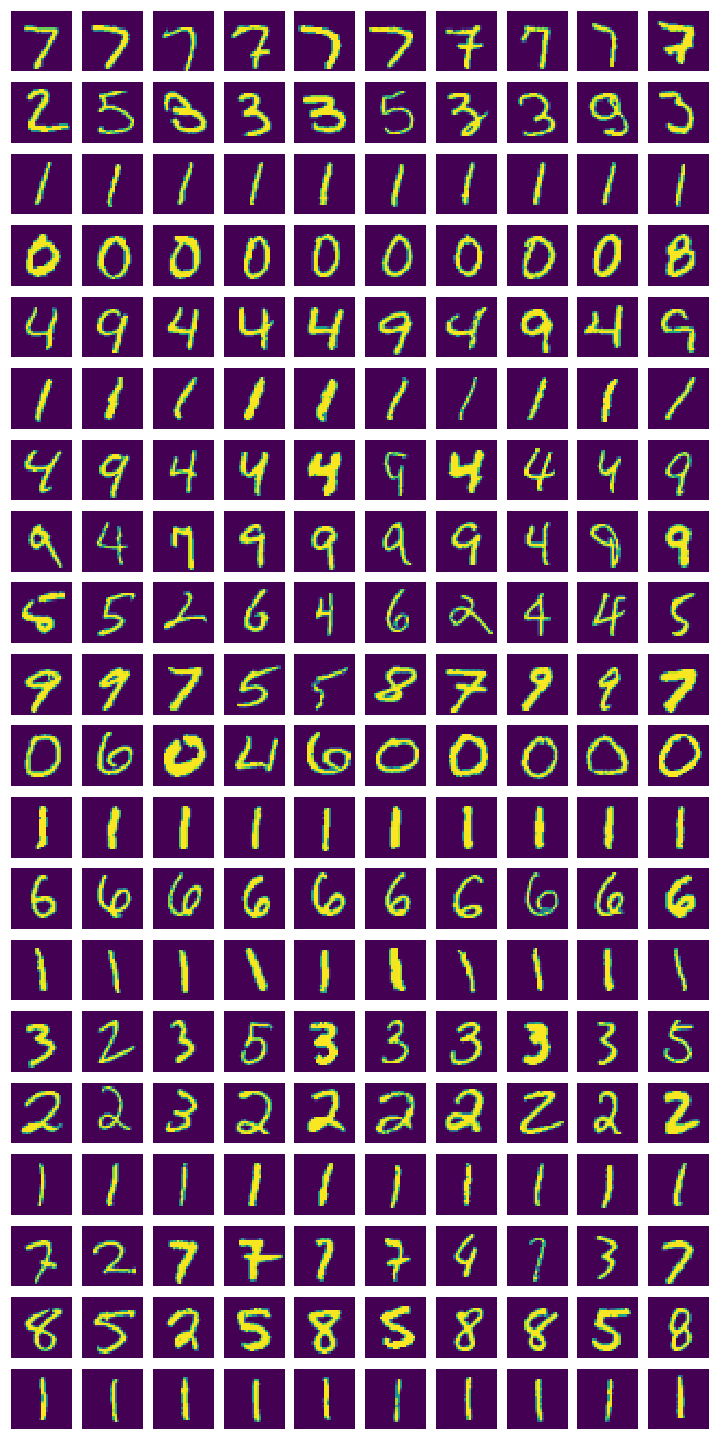
\includegraphics[height={0.6\textheight}]{../../images/number_clustering_20_2norm.png}
				\caption{Inverse of 2-norm of the difference vector between two images as similarity measure}
				\label{fig:clustering_20_2norm}
			\end{subfigure}
		\end{center}
		\caption{2000 images from MNIST data-set were clustered into 20 clusters. In the above figure, each row of images represent a cluster and show the first 10 images in that cluster}
		\label{fig:mnistImages}
	\end{figure}
	\end{frame}

	\begin{frame}{Spectral Clustering}
		\framesubtitle{Practical Considerations}
		\begin{itemize}
			\item Choice of Similarity Function
			
		\end{itemize}

	
	\nocite{govl:96, parlet:98,stsu:90,gene:2018}
	\frametitle{References}

	\bibliographystyle{unsrt}
	\bibliography{long_string, Mybib} 
	
\end{document}